\chapter{Layout \& Configuration}
\label{ch:layo_and_conf}

This chapter elaborates on the layout and internal configuration of the Winged Quadcopter; the concept that was finally selected based on the score in the trade-off. \autoref{sec:exte_inte_layo} contains isometric and top view drawings of the external and internal layout of the concept. The drawings give an indication of the location of the main subsystems, such as the battery unit, payload bay and communication system. \autoref{secCF} presents the communication flow, which is the exchange of information between different subsystems and the environment.

\section{External and Internal Layout}
\label{sec:exte_inte_layo}

\autoref{fig:iso_view_ext} shows the external isometric view of the Winged Quadcopter.

\begin{figure}[htb]
\includegraphics[width=\textwidth]{./LayoutConfiguration/Figures/iso_view}
\caption{Isometric external view of the Winged Quadcopter}
\label{fig:iso_view_ext}
\end{figure}

\autoref{fig:top_view_lay} presents the top view of the internal layout of the main components. It should be noted that the battery and computer are position above the payload bay.

\begin{figure}[htb]
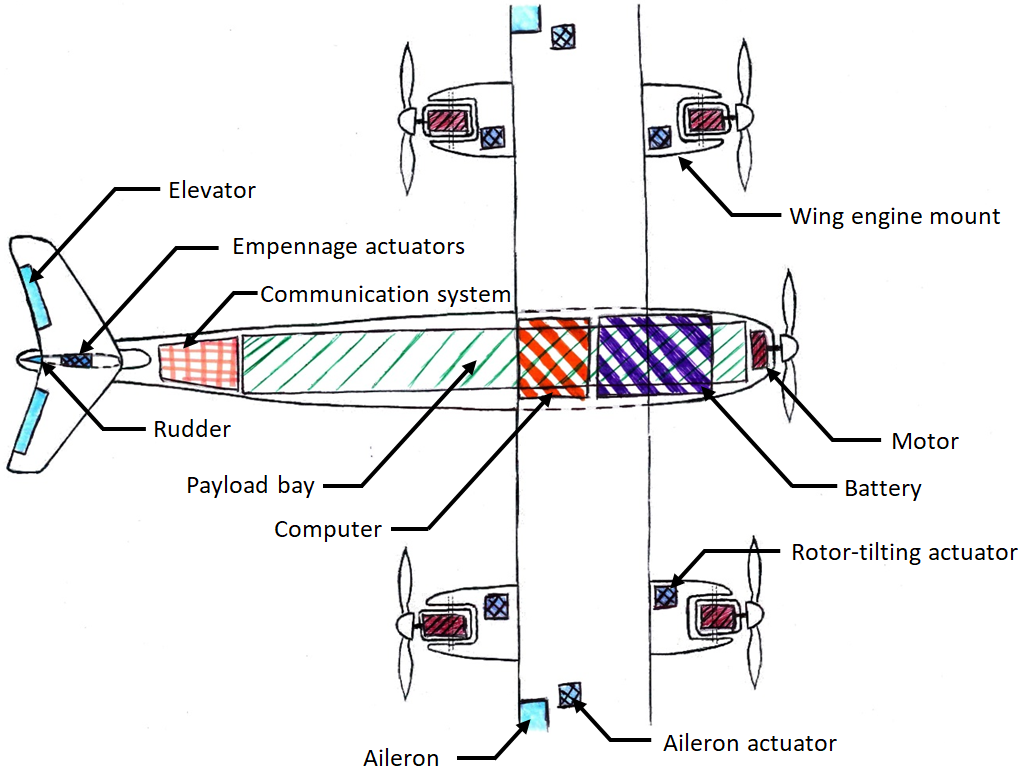
\includegraphics[width=\textwidth]{./LayoutConfiguration/Figures/top_view}
\caption{Top view internal layout of the Winged Quadcopter}
\label{fig:top_view_lay}
\end{figure}

\section{Communication Flow}
\label{secCF}
The communication flow diagram presented in this chapter is a tool that helps visualise the flow of information and commands through the UAV and between the UAV and the environment. Central to this communication flow diagram is the on-board CPU. The on-board CPU, in addition to processing the data received from both the sensors and the GPS satellites, serves as a hub through which information flows.

Not all of what is included in this communication flow is necessary for all missions. For example, depending on where the UAV is operated (over land, offshore, central or remote) communication with the ground station can take place via cellular connection or via satellite communication. The requisite systems can therefore be adapted on a per mission basis.

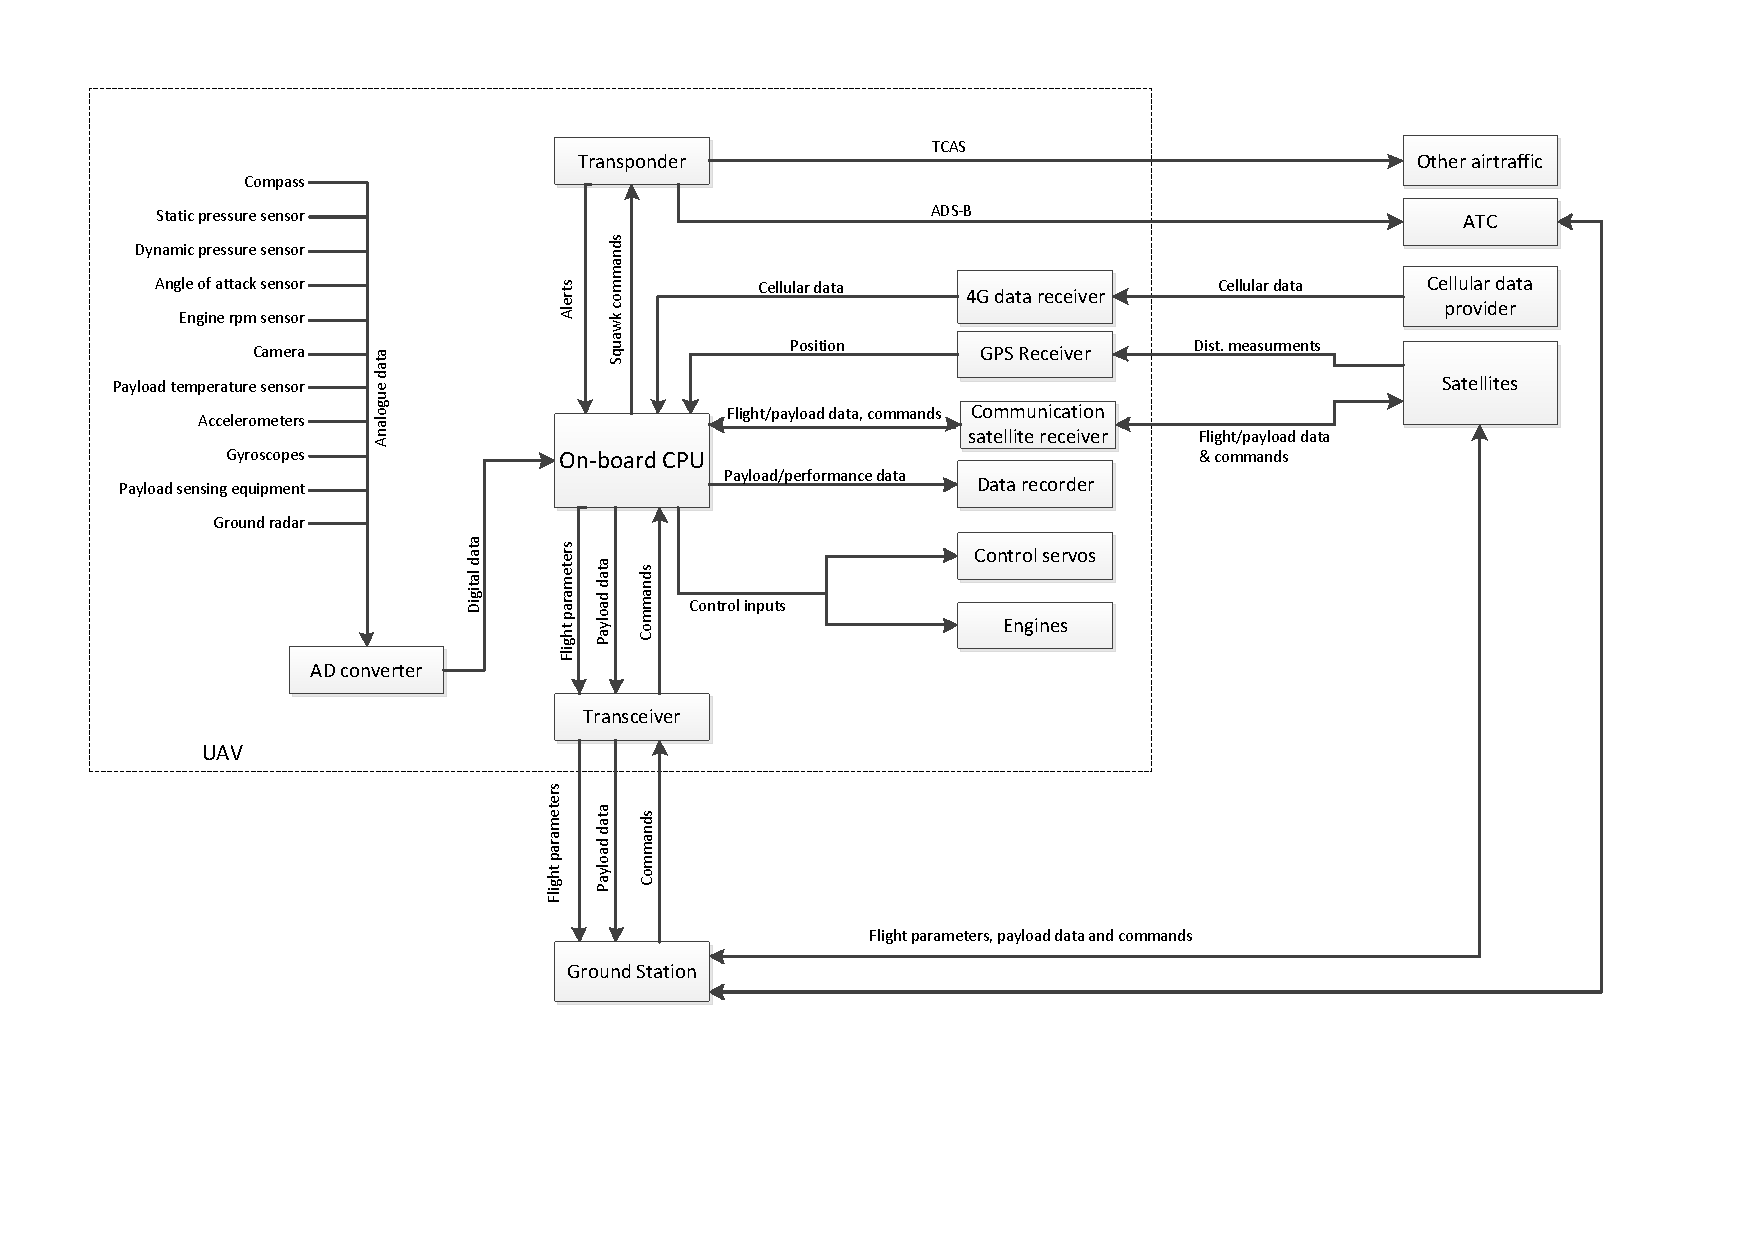
\includepdf[pages=1,fitpaper, scale=0.85,pagecommand={}]{LayoutConfiguration/Figures/CFD.pdf}